\DeclareSong{Tall Tale No. 5}{Patients}{Volume 1}%[Capo]
\intro{G}
\begin{strophe*}
  \begin{tabular}{l l}
   Oh, I was \chord[c]{G}born on a \chord[c]{D}Sunday &
   With \chord[c]{C}blood on my \chord[c]{G}hands \tbnl
   
   In a \chord[c]{C}room full of \chord[c]{G}photographs & 
   And \chord[c]{D}old electric fans \tbnl
   
   And I \chord[c]{G}slept in a \chord[c]{D}graveyard &
   For \chord[c]{C}bicycles and \chord[c]{G}cars \tbnl
   
   And I \chord[c]{C}dreamed of distant \chord[c]{G}scenery & 
   But \chord[c]{D}never strayed too far \\[1em]
   
   'cause I \chord[c]{C}do what they \chord[c]{G}ask me & 
   I \chord[c]{C}never run my \chord[c]{G}mouth \tbnl
   
   And by the \chord[c]{C}time you turn a\chord[c]{G}gainst me &
   I'll \chord[c]{D}have you figured out
  \end{tabular}
\end{strophe*}
\vskip 0.5em
\begin{chorus*}
  And \chord[c]{G}I\pause \chord[c]{C}learned to \chord[c]{G}lie
  
  By watching you \chord[c]{C}turn to your \chord[c]{G}enemies
  
  And the apple you've \chord[c]{C}got in your \chord[c]{G}eye
  
  Has be\chord[c]{Em}come a \chord[c]{C}stain, you don't \chord[c]{D}want it
\end{chorus*}
\vskip 0.5em
\begin{strophe*}
  \begin{tabular}{l l}
   So I \chord[c]{G}left for the \chord[c]{D}city &
   As \chord[c]{C}soon as I could \chord[c]{G}walk \tbnl
   
   But the \chord[c]{C}buildings loomed like \chord[c]{G}sentinels &
   It \chord[c]{D}wasn't what I thought \tbnl
   
   So I \chord[c]{G}slept in your \chord[c]{D}bathtub & 
   While you \chord[c]{C}put your make-up \chord[c]{G}on \tbnl
   
   And I \chord[c]{C}day-dreamed a\chord[c]{G}bout your lungs & 
   'til your \chord[c]{D}cigarettes were gone\\[1em]
   
   Now I \chord[c]{C}wrote 'cause I \chord[c]{G}have to & 
   I'm \chord[c]{C}never welcome \chord[c]{G}home \tbnl
   
   And though this \chord[c]{C}road leads to di\chord[c]{G}saster &
   I've \chord[c]{D}always got my songs
  \end{tabular}
\end{strophe*}
\vskip 0.5em
\begin{chorus*}
  And \chord[c]{G}I\pause \chord[c]{C}learned to \chord[c]{G}laugh \pause (ha ha ha ha)
  
  By watching you \chord[c]{C}burn all your \chord[c]{G}photographs
  
  And you're right that the \chord[c]{C}good stuff won't \chord[c]{G}last
  
  But these \chord[c]{Em}wars are never \chord[c]{C}won by our \chord[c]{D}twiddling \chord[c]{G}thumbs
\end{chorus*}
\interlude{C\pause G\rep{3}\pause D\Pause C\pause G\rep{3}\pause D}
\begin{strophe*}
  \begin{tabular}{l l}
   Well, I \chord[c]{C}did what they \chord[c]{G}asked me & 
   I \chord[c]{C}never ran my \chord[c]{G}mouth \tbnl
   
   And by the \chord[c]{C}time they turned a\chord[c]{G}gainst me & 
   I \chord[c]{D}had them figured out \\[1em]
   
   And now I \chord[c]{C}wrote 'cause I \chord[c]{G}have to & 
   I'm \chord[c]{C}never welcome \chord[c]{G}home \tbnl
   
   And though this \chord[c]{C}road leads to di\chord[c]{G}saster &
   I've \chord[c]{D}always got my songs
  \end{tabular}
\end{strophe*}
\begin{chorus*}
  And \chord[c]{G}I\pause \chord[c]{C}learned to \chord[c]{G}die
  
  By watching you \chord[c]{C}choke on your \chord[c]{G}miseries
  
  And if the apple gets \chord[c]{C}torn from my \chord[c]{G}eye
  
  Well, I \chord[c]{Em}won't be a\chord[c]{C}lone 'cause I'm \chord[c]{D}going \chord[c]{G}home
\end{chorus*}

\vfill
\begin{center}
 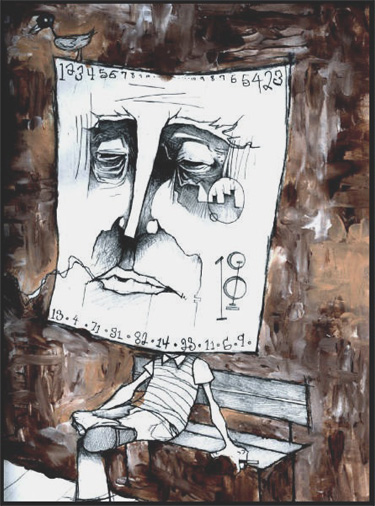
\includegraphics[scale=3]{pni33.jpg}
\end{center}
\vfill